\documentclass[a4paper, 11pt]{article}
\usepackage[python,linenum]{mypackage}
\usepackage{amsmath}
\usepackage{graphicx}
\usepackage{geometry}
\geometry{scale=0.8}
\usepackage{hyperref}
\usepackage{enumitem}
\usepackage{color}
\usepackage[linesnumbered,boxed]{algorithm2e}

\setenumerate[1]{itemsep=0pt,partopsep=0pt,parsep=\parskip,topsep=0pt}
\setitemize[1]{itemsep=0pt,partopsep=0pt,parsep=\parskip,topsep=0pt}
\setdescription{itemsep=0pt,partopsep=0pt,parsep=\parskip,topsep=0pt}


\title{
\normalfont \normalsize
\textsc{School of Data and Computer Science, Sun Yat-sen University} \\ [25pt] %textsc small capital letters
\rule{\textwidth}{0.5pt} \\[0.4cm] % Thin top horizontal rule
\huge  E15 Reinforcement Learning (C++/Python)\\ % The assignment title
\rule{\textwidth}{2pt} \\[0.5cm] % Thick bottom horizontal rule
\author{17341015 Hongzheng Chen}
\date{\normalsize\today}
}

\begin{document}
\maketitle
\tableofcontents
\newpage
\section{Overview}
\begin{figure}[H]
\centering
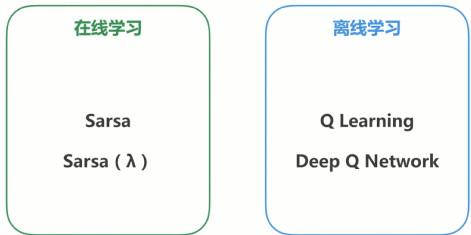
\includegraphics[width=8cm]{fig/on_off}
\quad
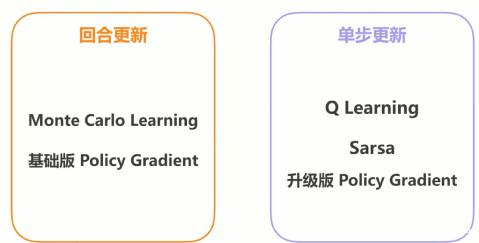
\includegraphics[width=8cm]{fig/update}
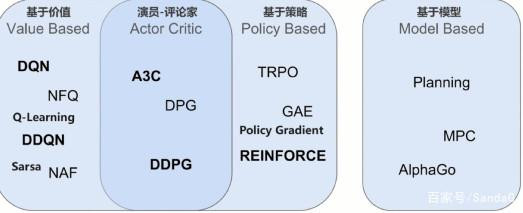
\includegraphics[width=11cm]{fig/base}
\quad
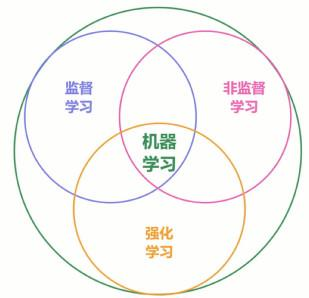
\includegraphics[width=5cm]{fig/relation}
\end{figure}
\section{Tutorial}
English version: \url{http://mnemstudio.org/path-finding-q-learning-tutorial.htm}\\
Chinese version: \url{https://blog.csdn.net/itplus/article/details/9361915}
\subsection{Step-By-Step Tutorial}
Suppose we have 5 rooms in a building connected by doors as shown in the figure below.  We'll number each room 0 through 4.  The outside of the building can be thought of as one big room (5).  Notice that doors 1 and 4 lead into the building from room 5 (outside). We can represent the rooms on a graph, each room as a node, and each door as a link.


For this example, we'd like to put an agent in any room, and from that room, go outside the building (this will be our target room). In other words, the goal room is number 5. To set this room as a goal, we'll associate a reward value to each door (i.e. link between nodes). The doors that lead immediately to the goal have an instant reward of 100.  Other doors not directly connected to the target room have zero reward. Because doors are two-way ( 0 leads to 4, and 4 leads back to 0 ), two arrows are assigned to each room. Each arrow contains an instant reward value, as shown below:

\begin{figure}[H]
\centering
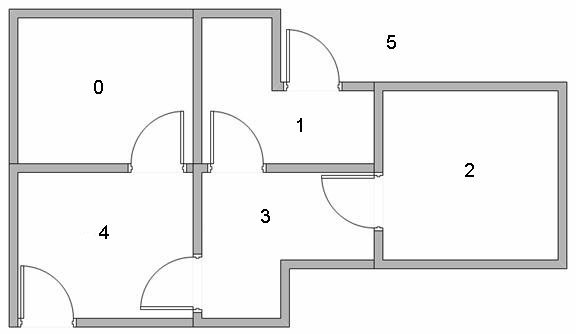
\includegraphics[width=8cm]{fig/modeling_environment_clip_image002a}
\quad
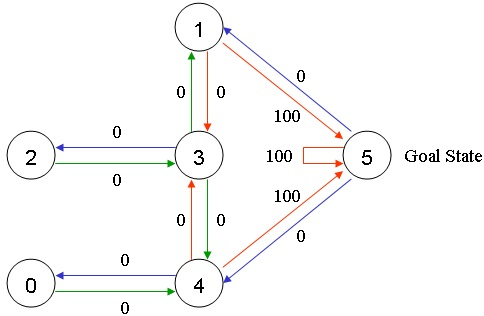
\includegraphics[width=8cm]{fig/map2a}
\end{figure}

Of course, Room 5 loops back to itself with a reward of 100, and all other direct connections to the goal room carry a reward of 100.  In Q-learning, the goal is to reach the state with the highest reward, so that if the agent arrives at the goal, it will remain there forever. This type of goal is called an "absorbing goal".

Imagine our agent as a dumb virtual robot that can learn through experience. The agent can pass from one room to another but has no knowledge of the environment, and doesn't know which sequence of doors lead to the outside.

Suppose we want to model some kind of simple evacuation of an agent from any room in the building. Now suppose we have an agent in Room 2 and we want the agent to learn to reach outside the house (5).

The terminology in Q-Learning includes the terms "state" and "action".

We'll call each room, including outside, a "state", and the agent's movement from one room to another will be an "action".  In our diagram, a "state" is depicted as a node, while "action" is represented by the arrows.

\begin{figure}[H]
\centering
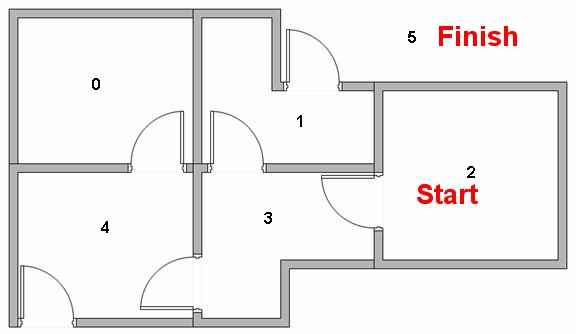
\includegraphics[width=8cm]{fig/agent_clip_image002}
\quad
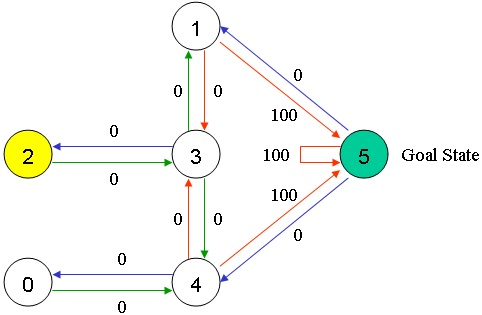
\includegraphics[width=8cm]{fig/map3a}
\end{figure}

Suppose the agent is in state 2.  From state 2, it can go to state 3 because state 2 is connected to 3.  From state 2, however, the agent cannot directly go to state 1 because there is no direct door connecting room 1 and 2 (thus, no arrows).  From state 3, it can go either to state 1 or 4 or back to 2 (look at all the arrows about state 3).  If the agent is in state 4, then the three possible actions are to go to state 0, 5 or 3.  If the agent is in state 1, it can go either to state 5 or 3.  From state 0, it can only go back to state 4.

We can put the state diagram and the instant reward values into the following reward table, "matrix R".

\begin{figure}[H]
\centering
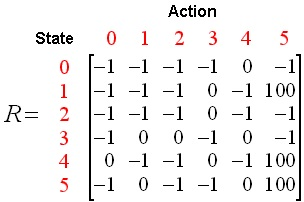
\includegraphics[width=7cm]{fig/r_matrix1}
\caption*{The -1's in the table represent null values (i.e.; where there isn't a link between nodes). }
\end{figure}

Now we'll add a similar matrix, "Q", to the brain of our agent, representing the memory of what the agent has learned through experience.  The rows of matrix Q represent the current state of the agent, and the columns represent the possible actions leading to the next state (the links between the nodes).

The agent starts out knowing nothing, the matrix Q is initialized to zero.  In this example, for the simplicity of explanation, we assume the number of states is known (to be six).  If we didn't know how many states were involved, the matrix Q could start out with only one element.  It is a simple task to add more columns and rows in matrix Q if a new state is found.

The transition rule of Q learning is a very simple formula:
$$Q(stte,action)=R(state,action)+\gamma\max[Q(next state,allactions)]$$

According to this formula, a value assigned to a specific element of matrix Q, is equal to the sum of the corresponding value in matrix R and the learning parameter $\gamma$, multiplied by the maximum value of Q for all possible actions in the next state.

Our virtual agent will learn through experience, without a teacher (this is called unsupervised learning).  The agent will explore from state to state until it reaches the goal. We'll call each exploration an episode.  Each episode consists of the agent moving from the initial state to the goal state.  Each time the agent arrives at the goal state, the program goes to the next episode.

The Q-Learning algorithm goes as follows:


  \begin{algorithm}
%
     \caption{The Q-Learning Algorithm}
       Set the gamma parameter, and environment rewards in matrix R\;
        Initialize matrix Q to zero\;
        \ForEach{episode}
        {
            Select a random initial state\;
            \While{ the goal state hasn’t been reached}
            {
                Select one among all possible actions for the current state\;
				Using this possible action, consider going to the next state\;
				Get maximum Q value for this next state based on all possible actions\;
				Compute: $Q(state, action) = R(state, action) + \gamma\max[Q(next state, all actions)]$\;
				Set the next state as the current state\;
            }
        }

    \end{algorithm}

The algorithm above is used by the agent to learn from experience.  Each episode is equivalent to one training session.  In each training session, the agent explores the environment (represented by matrix R ), receives the reward (if any) until it reaches the goal state. The purpose of the training is to enhance the 'brain' of our agent, represented by matrix Q.  More training results in a more optimized matrix Q.  In this case, if the matrix Q has been enhanced, instead of exploring around, and going back and forth to the same rooms, the agent will find the fastest route to the goal state.

The $\gamma$ parameter has a range of 0 to 1 ($0\leq\gamma<1$).  If $\gamma$ is closer to zero, the agent will tend to consider only immediate rewards.  If $\gamma$ is closer to one, the agent will consider future rewards with greater weight, willing to delay the reward.

To use the matrix Q, the agent simply traces the sequence of states, from the initial state to goal state.  The algorithm finds the actions with the highest reward values recorded in matrix Q for current state:

Algorithm to utilize the Q matrix:

1. Set current state = initial state.

2. From current state, find the action with the highest Q value.

3. Set current state = next state.

4. Repeat Steps 2 and 3 until current state = goal state.

The algorithm above will return the sequence of states from the initial state to the goal state.
\subsection{Q-learning Example By Hand}
To understand how the Q-learning algorithm works, we'll go through a few episodes step by step. The rest of the steps are illustrated in the source code examples.

We'll start by setting the value of the learning parameter $\gamma=0.8$, and the initial state as Room 1. Initialize matrix Q as a zero matrix. Look at the second row (state 1) of matrix R.  There are two possible actions for the current state 1: go to state 3, or go to state 5. By random selection, we select to go to 5 as our action.

\begin{figure}[H]
\centering
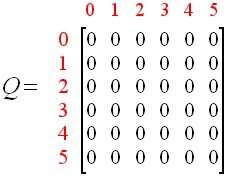
\includegraphics[width=7cm]{fig/q_matrix1}
\quad
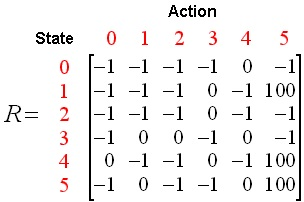
\includegraphics[width=7cm]{fig/r_matrix1}
\end{figure}
Now let's imagine what would happen if our agent were in state 5.  Look at the sixth row of the reward matrix R (i.e. state 5).  It has 3 possible actions: go to state 1, 4 or 5.
$$Q(state, action) = R(state, action) + \gamma\max[Q(next state, all actions)]$$
$$Q(1, 5) = R(1, 5) + 0.8\times\max[Q(5, 1), Q(5, 4), Q(5, 5)] = 100 + 0.8\times 0 = 100$$

Since matrix Q is still initialized to zero, Q(5, 1), Q(5, 4), Q(5, 5), are all zero.  The result of this computation for Q(1, 5) is 100 because of the instant reward from R(5, 1).

The next state, 5, now becomes the current state.  Because 5 is the goal state, we've finished one episode.  Our agent's brain now contains an updated matrix Q as:

\begin{figure}[H]
\centering
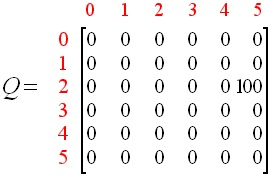
\includegraphics[width=7cm]{fig/q_matrix2}
\end{figure}

For the next episode, we start with a randomly chosen initial state.  This time, we have state 3 as our initial state.

Look at the fourth row of matrix R; it has 3 possible actions: go to state 1, 2 or 4.  By random selection, we select to go to state 1 as our action.

Now we imagine that we are in state 1.  Look at the second row of reward matrix R (i.e. state 1).  It has 2 possible actions: go to state 3 or state 5.  Then, we compute the Q value:
$$Q(state, action) = R(state, action) + \gamma\max[Q(next state, all actions)]$$
$$Q(1, 5) = R(1, 5) + 0.8\times\max[Q(1, 2), Q(1, 5)] = 0 + 0.8\times\max(0, 100) = 80$$

We use the updated matrix Q from the last episode.  Q(1, 3) = 0 and Q(1, 5) = 100.  The result of the computation is Q(3, 1) = 80 because the reward is zero.  The matrix Q becomes:
\begin{figure}[H]
\centering
\centering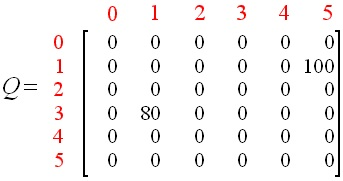
\includegraphics[width=7cm]{fig/q_matrix3}
\end{figure}

The next state, 1, now becomes the current state.  We repeat the inner loop of the Q learning algorithm because state 1 is not the goal state.

So, starting the new loop with the current state 1, there are two possible actions: go to state 3, or go to state 5.  By lucky draw, our action selected is 5.

\begin{figure}[H]
\centering
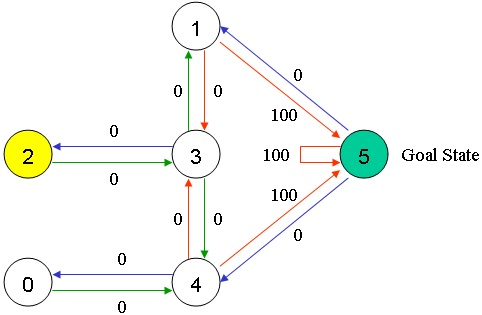
\includegraphics[width=7cm]{fig/map3a}
\end{figure}

Now, imaging we're in state 5, there are three possible actions: go to state 1, 4 or 5.  We compute the Q value using the maximum value of these possible actions.

$$Q(state, action) = R(state, action) + \gamma\max[Q(next state, all actions)]$$

$$Q(1, 5) = R(1, 5) + 0.8 \times\max[Q(5, 1), Q(5, 4), Q(5, 5)] = 100 + 0.8\times0 = 100$$

The updated entries of matrix Q, Q(5, 1), Q(5, 4), Q(5, 5), are all zero.  The result of this computation for Q(1, 5) is 100 because of the instant reward from R(5, 1).  This result does not change the Q matrix.

Because 5 is the goal state, we finish this episode.  Our agent's brain now contain updated matrix Q as:

\begin{figure}[H]
\centering
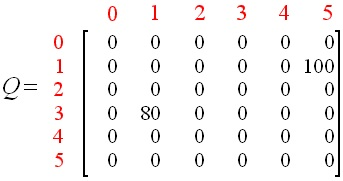
\includegraphics[width=7cm]{fig/q_matrix3}
\end{figure}

If our agent learns more through further episodes, it will finally reach convergence values in matrix Q like:

\begin{figure}[H]
\centering
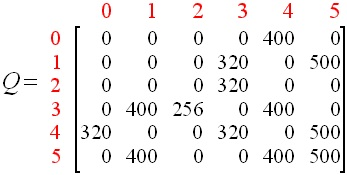
\includegraphics[width=7cm]{fig/q_matrix4}
\end{figure}

This matrix Q, can then be normalized (i.e.; converted to percentage) by dividing all non-zero entries by the highest number (500 in this case):

\begin{figure}[H]
\centering
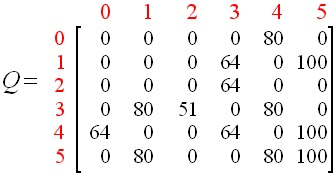
\includegraphics[width=7cm]{fig/q_matrix5}
\end{figure}

Once the matrix Q gets close enough to a state of convergence, we know our agent has learned the most optimal paths to the goal state.  Tracing the best sequences of states is as simple as following the links with the highest values at each state.

\begin{figure}[H]
\centering
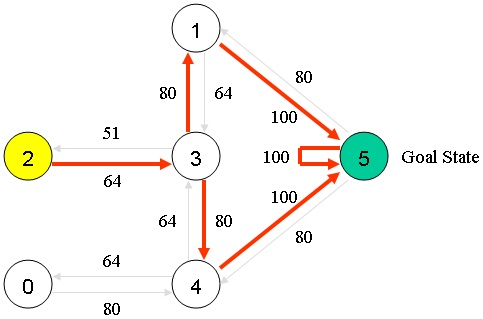
\includegraphics[width=7cm]{fig/map5}
\end{figure}

For example, from initial State 2, the agent can use the matrix Q as a guide:

From State 2 the maximum Q values suggests the action to go to state 3.

From State 3 the maximum Q values suggest two alternatives: go to state 1 or 4.  Suppose we arbitrarily choose  to go to 1.

From State 1 the maximum Q values suggests the action to go to state 5.

Thus the sequence is 2 - 3 - 1 - 5.

\section{Flappy Bird}
\begin{figure}[H]
\centering

\includegraphics[width=11cm]{fig/bird}
\end{figure}
Flappy Bird was a side-scrolling mobile game, the objective was to direct a flying bird, named "Faby", who moves continuously to the right, between sets of Mario-like pipes. Note that the pipes always have the same gap between them and there is no end to the running track. If the player touches the pipes, they lose. Faby briefly flaps upward each time that the player taps the screen; if the screen is not tapped, Faby falls because of gravity; each pair of pipes that he navigates between earns the player a single point, with medals awarded for the score at the end of the game. Android devices enabled the access of world leaderboards, through Google Play. You can also play this game on-line: \url{http://flappybird.io/}.


\section{Tasks}
\begin{enumerate}
	\item \textcolor{blue}{\textbf{Implement the algorithm in the tutorial example ,and output the Q-matrix and the path with the highest values.}}
	\item Now here is a flappy bird project (Python3) for you, and the file \texttt{bot.py} is incomplete. You should implement a flappy bird bot who learns from each game played via Q-learning.

	Please pay attention to the following points:
	\begin{itemize}
		\item The state of the bird is defined by the horizontal and vertical distances fro the next pipe and the velocity of the bird.
		\item In order to understand the state space, you need to briefly understand the following sizes: \texttt{SCREENWIDTH=288,SCREENHEIGHT=512, PIPEGAPSIZE=100, BASEY=SCREENHEIGHT*0.79, PIPE=[52,320],PLAYER=[34,24],BASE=[336,112], BACKGROUND=[288,512],etc.}
		\item The Q values are dumped to the local JSON file \texttt{qvalues.json}.
		\item \texttt{initialize\_qvalues.py} is an independent file, and we can run \texttt{python initialize\_qvalues.py} to initialize the Q values. Of course, this file has been initialized.
		\item You can run \texttt{python learn.py --verbose 5000} to update the Q values dumped to \texttt{qvalues.json} with 5000 iterations, and then run \texttt{python flappy.py} to observe the performance the bird.
	\end{itemize}
	\textcolor{blue}{\textbf{Please complete the function \texttt{update\_scores()} in \texttt{bot.py}, and run \texttt{python learn.py --verbose 5000} and \texttt{python learn.py --verbose 10000} to get the following figures, respectively.}}
	\begin{figure}[H]
	\centering
	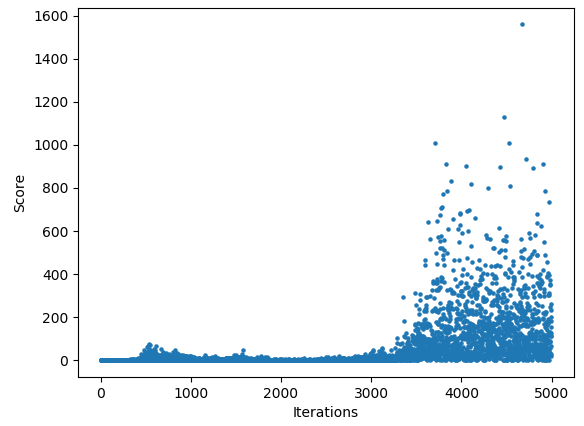
\includegraphics[width=8cm]{fig/score5000}
	\quad
	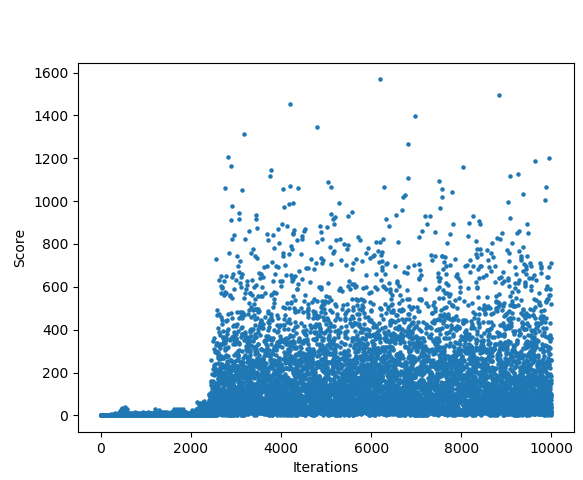
\includegraphics[width=8cm]{fig/score10000}
	\end{figure}
	\item Please submit a file named \texttt{E15\_YourNumber.pdf} and send it to \texttt{ai\_201901@foxmail.com}
\end{enumerate}

\section{Codes and Results}
The results are shown below, the left figure for 5000 training iterations, and the right one for 10000 iterations.
\begin{figure}[H]
\centering
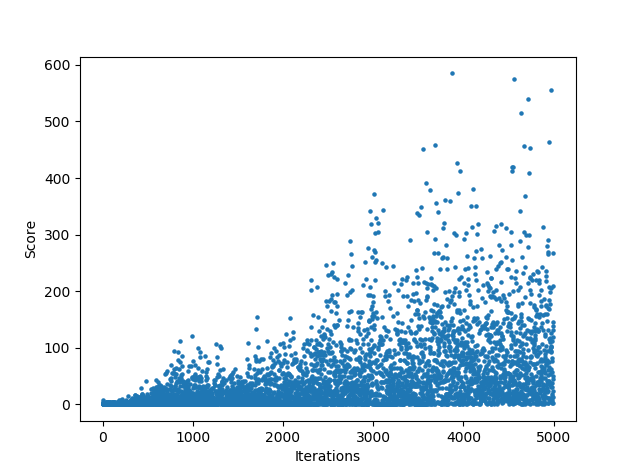
\includegraphics[width=8cm]{fig/result1.png}
\quad
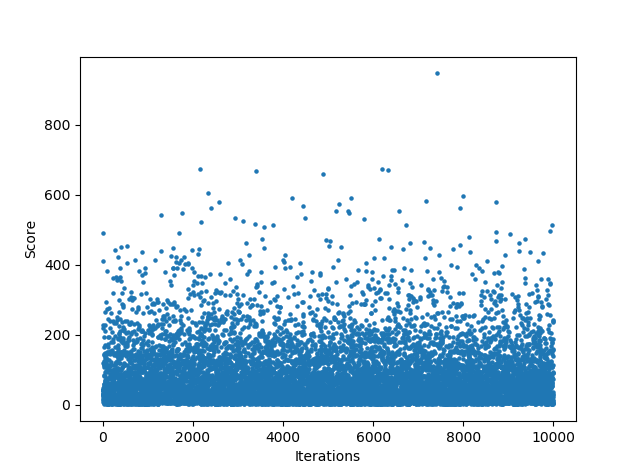
\includegraphics[width=8cm]{fig/result2.png}
\end{figure}

Following only gives the \verb'update_scores' function, for the whole program, please refer to \verb'bot.py'.
\begin{lstlisting}
def update_scores(self, dump_qvalues = True):
	"""
	Update qvalues via iterating over experiences
	"""
	history = list(reversed(self.moves))

	# Flag if the bird died in the top pipe
	high_death_flag = True if int(history[0][2].split("_")[1]) > 120 else False

	# Q-learning score updates
	for i,(last_state, action, state) in enumerate(history):

		# Select reward
		# 0: still alive  1: game over
		if i in [0,1]:
			# last state has been the "game over" state
			# thus the last second that leads to the "game over" state should also receive negative rewards
			reward = self.r[1]
		elif high_death_flag and action == 1:
			# if the bird died in the top pipe
			# then the previous action should be 1 (flip up)
			reward = self.r[1]
			high_death_flag = False
		else:
			# otherwise, the bird is alive
			reward = self.r[0]

		# find the max q value
		maxq = max(self.qvalues[state][0],self.qvalues[state][1])

		# Update self.qvalues[state][act]
		# Balance exploitation and exploration
		self.qvalues[last_state][action] = (1 - self.lr) * self.qvalues[last_state][action] + self.lr * (reward + self.discount * maxq)

	self.gameCNT += 1  # increase game count
	if dump_qvalues:
		self.dump_qvalues()  # Dump q values (if game count % DUMPING_N == 0)
	self.moves = []  # clear history after updating strategies
\end{lstlisting}

\end{document}